\documentclass[a4paper,12pt]{article}
\usepackage{graphicx}
\usepackage{tikz}
\usetikzlibrary{shapes.geometric, arrows}
\usepackage[utf8]{inputenc}
\usepackage[T2A]{fontenc}
\usepackage[english,russian]{babel}
\usepackage{natbib}
\usepackage{graphicx}
\usepackage{amsmath}
\usepackage{pgfplots}
\usepackage{pdfpages}
\usepackage[unicode, pdftex]{hyperref}
\pgfplotsset{compat=newest}
\usepackage{color} %% это для отображения цвета в коде
\usepackage{listings} %% собственно, это и есть пакет listings
\usepackage{caption}
\DeclareCaptionFont{white}{\color{white}} %% это сделает текст заголовка белым
%% код ниже нарисует серую рамочку вокруг заголовка кода.
\DeclareCaptionFormat{listing}{\colorbox{white}{\parbox{\textwidth}{#1#2#3}}}
\captionsetup[lstlisting]{format=listing,labelfont=black,textfont=black}

%%%%%%%%%%%%%%%%%%%%%%%%%%%%%%%%%%%%%%%%%%%%%%%%%%%%%%%%%%%%%%%%%%%%%%%%%%%%%%%%%%%%%%%%%%%%%%%

\begin{document}
	\lstset{ %
        language=C,                % выбор языка для подсветки (здесь это С)
        basicstyle=\small\sffamily, % размер и начертание шрифта для подсветки кода
        numbers=left,               % где поставить нумерацию строк (слева\справа)
        numberstyle=\tiny,           % размер шрифта для номеров строк
        stepnumber=1,                   % размер шага между двумя номерами строк
        numbersep=-5pt,                % как далеко отстоят номера строк от         подсвечиваемого кода
        backgroundcolor=\color{white}, % цвет фона подсветки - используем         \usepackage{color}
        showspaces=false,            % показывать или нет пробелы специальными     отступами
        showstringspaces=false,      % показывать или нет пробелы в строках
        showtabs=false,             % показывать или нет табуляцию в строках
        frame=single,              % рисовать рамку вокруг кода
        tabsize=2,                 % размер табуляции по умолчанию равен 2 пробелам
        captionpos=t,              % позиция заголовка вверху [t] или внизу [b] 
        breaklines=true,           % автоматически переносить строки (да\нет)
        breakatwhitespace=false, % переносить строки только если есть пробел
        escapeinside={\%*}{*)},   % если нужно добавить комментарии в коде
	    keywordstyle=\color{blue}\ttfamily,
	    stringstyle=\color{red}\ttfamily,
	    commentstyle=\color{green}\ttfamily,
	    morecomment=[l][\color{magenta}]{\#},
	    columns=fullflexible
    }
\thispagestyle{empty}

\begin{figure}[th]
\noindent\centering{

\includepdf[pages=-]{title.pdf}}
\end{figure}

%%%%%%%%%%%%%%%%%%%%%%%%%%%%%%%%%%%%%%%%%%%%%%%%%%%%%%%%%%%%%%%%%%%%%%%%%%%%%%%%%%%%%%%%%%%%%%%
\newpage
\textbf {Задание}\\

В лабораторной работе анализируется результат выполнения трех программ. Программы демонстрируют открытие одного и того же файла несколько раз. Реализация открытия файла в одной программе несколько раз выбрана для простоты. Такая ситуация возможна в системе, когда один и тот же файл несколько раз открывают разные процессы. Но для получения ситуаций аналогичных тем, которые демонстрируют приведенные программы надо было бы синхронизировать работу процессов. При выполнении асинхронных процессов такая ситуация вероятна и ее надо учитывать, чтобы избежать потери данных или получения неверного результата при выводе в файл.

\textbf {Первая программа:}
\begin{lstlisting}
  //testCIO.c
  #include <stdio.h>
  #include <fcntl.h>

  /*
  On my machine, a buffer size of 20 bytes
  translated into a 12-character buffer.
  Apparently 8 bytes were used up by the
  stdio library for bookkeeping.
   */

  int main()
  {
    // have kernel open connection to file alphabet.txt
    int fd = open("alphabet.txt",O_RDONLY);

    // create two a C I/O buffered streams using the above connection 
    FILE *fs1 = fdopen(fd,"r");
    char buff1[20];
    setvbuf(fs1,buff1,_IOFBF,20);

    FILE *fs2 = fdopen(fd,"r");
    char buff2[20];
    setvbuf(fs2,buff2,_IOFBF,20);
    
    // read a char & write it alternatingly from fs1 and fs2
    int flag1 = 1, flag2 = 2;
    while(flag1 == 1 || flag2 == 1)
    {
        char c;
        flag1 = fscanf(fs1,"%c",&c);
        if (flag1 == 1) 
        {
	          fprintf(stdout,"%c",c);
        }
        flag2 = fscanf(fs2,"%c",&c);
        if (flag2 == 1) 
        { 
	          fprintf(stdout,"%c",c); 
        }
    }
    return 0;
  }
\end{lstlisting}

\begin{figure}[th]
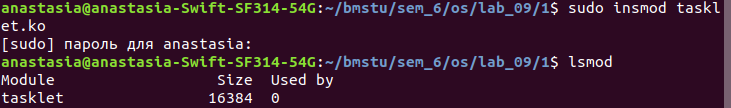
\includegraphics[scale = 0.9]{1.png}
\caption{Результат выполнения первой программы}
\label{ris:first}
\end{figure}

\textbf {Анализ полученного результата:}\\

Работа с содержимым файла происходит через целочисленный файловый дескриптор, который представляет из себя номер строки в таблице ссылок на открытые файлы процесса. При помощи системного вызова open() создается файловый дескриптор fd, файл открывается на чтение, указатель на текущую позицию в файле устанавливается на начало файла. Если системный  вызов  завершается  успешно,  возвращенный  файловый  дескриптор является самым маленьким дескриптором, который еще не открыт  процессом. Возвращается -1 в случае ошибки. Функция fdopen связывает два потока на чтение с существующим файловым дескриптором fd. Функция setvbuf задает блочную буферизацию с размером буфера 20 байт. \underline{ }IOFBF - полная буферизация, то есть данные будут буферизироваться, пока буфер не заполниться полностью. В цикле данные считываются из двух потоков fs1 и fs2 в стандартный поток вывода stdout. Так как открытые файлы, для которых используется ввод/вывод потоков, буферизуются и размер буфера 20 байт, то в поток fs1 будут считаны первые 20 символов и указатель на текущую позицию в файле будет смещён на 20. В поток fs2 будут считаны оставшиеся 6 символов и символ конца строки. Осуществляется поочередное чтение из двух потоков, через 7 итераций все данные из второго буфера будут считаны и будут выводиться только символы из первого буфера (символы hijklmnopqrst).
\\

\begin{figure}[th]
\includegraphics[scale = 0.65]{gr1.jpg}
\caption{Рисунок, демонстрирующий созданные дескрипторы и связь между ними}
\label{ris:gr1}
\end{figure}

\textbf {Вторая программа:}
\begin{lstlisting}
  //testKernelIO.c
  #include <fcntl.h>
  #include <unistd.h>

  int main()
  {
      char c;    
      // have kernel open two connection to file alphabet.txt
      int fd1 = open("alphabet.txt",O_RDONLY);
      int fd2 = open("alphabet.txt",O_RDONLY);
      // read a char & write it alternatingly from connections fs1 & fd2
      int fl = 1;

      while(fl)
      {
          fl = 0;
          if (read(fd1,&c,1))
          {
              write(1,&c,1);
              if (read(fd2,&c,1))
              {
                  write(1,&c,1);
                  fl = 1;
              }
          }
      }
      return 0;
  }
\end{lstlisting}

\begin{figure}[th]
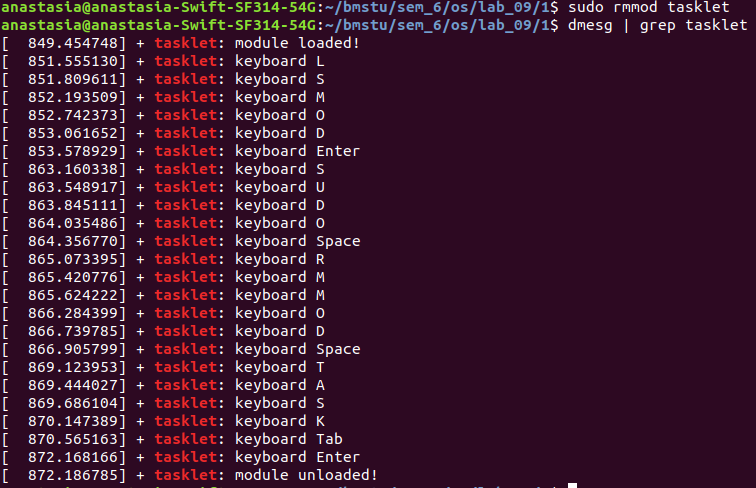
\includegraphics[scale = 0.9]{2.png}
\caption{Результат выполнения второй программы}
\label{ris:second}
\end{figure}
\textbf {Анализ полученного результата:}\\

В данной программе с помощью системного вызова open() создаются два файловых дескриптора одного и того же файла, открытого на чтение, то есть создаются две разные записи в системной таблице открытых файлов. Каждая запись будет иметь свою текущую позицию в файле, то есть положения указателей в файле независимы друг от друга. Системные вызовы read(), write() предоставляют небуферизованный ввод-вывод. Ввод-вывод является небуферизованным в том смысле, что каждый вызов read, write делает системный вызов в ядро ОС. В цикле при помощи системных вызовов read() и write() считывается символ из файла и этот символ записывается два раза в stdout, так как указатели в файле независимы друг от друга.
\\
\begin{figure}[th]
\includegraphics[scale = 0.65]{gr2.jpg}
\caption{Рисунок, демонстрирующий созданные дескрипторы и связь между ними}
\label{ris:gr2}
\end{figure}

\newpage
\textbf {Третья программа:}
\begin{lstlisting}
  #include <fcntl.h>
  #include <stdio.h>

  int main() 
  {
      FILE *fs1 = fopen("q.txt", "w");
      FILE *fs2 = fopen("q.txt", "w");

      for(char c = 'a'; c <= 'z'; c++)
      {
	        if (c%2)
          {
	            fprintf(fs1, &c, 1);
	        }
    	    else
          {
	            fprintf(fs2, &c, 1);
	        }
      }
      fclose(fs1);
      fclose(fs2);
      return 0;
  }
\end{lstlisting}
 
\begin{figure}[th]
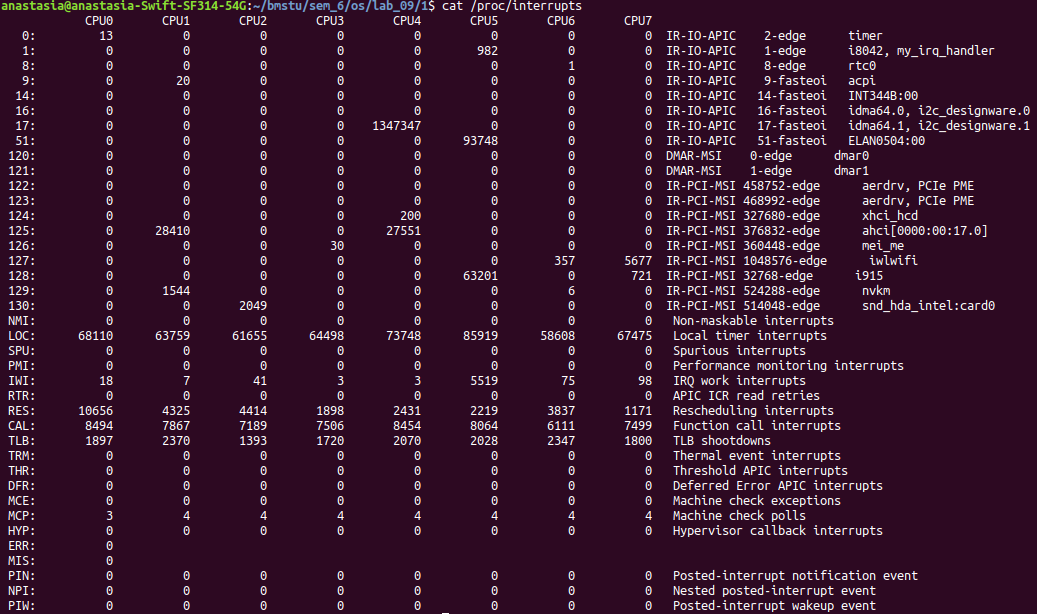
\includegraphics[scale = 0.9]{3.png}
\caption{Результат выполнения третьей программы}
\label{ris:third}
\end{figure}
\textbf {Анализ полученного результата:}\\

С помощью fopen() открываются два потока на запись, которые имеют разные файловые дескрипторы. Нечётные буквы алфавита записываются в первый поток fs1, чётные - во второй fs2. Так как функция fopen() выполняет ввод-вывод с буферизацией, окончательная запись в файл осуществляется либо при полном заполнении буфера, либо при вызове функций fclose() или функции fflush(). Если поток использовался для вывода данных, то после вызова fclose() все данные, содержащиеся в буфере, записываются в файл с помощью fflush().Так как поток fs1 использовался для вывода данных, после вызова fclose(fs1) все данные записываются из буфера в файл. При этом поток остается открытым. Так как используются два различных файловых дескриптора, то их указатели на текущую позицию в файле независимы, поэтому при вызове fclose(fs2) данные из второго буфера записываются в файл с начальной позиции, таким образом затирая данные записанные ранее из первого буфера. В итоге в файл будут записаны чётные буквы алфавита - bdfhjlnprtvxz.
\\

\begin{figure}[th]
\includegraphics[scale = 0.65]{gr3.jpg}
\caption{Рисунок, демонстрирующий созданные дескрипторы и связь между ними}
\label{ris:gr3}
\end{figure}

\newpage

\textbf {Структура FILE}\\
\begin{lstlisting}
  struct _IO_FILE {
    int _flags;		/* High-order word is _IO_MAGIC; rest is flags. */
  #define _IO_file_flags _flags

    /* The following pointers correspond to the C++ streambuf protocol. */
    /* Note:  Tk uses the _IO_read_ptr and _IO_read_end fields directly. */
    char* _IO_read_ptr;	/* Current read pointer */
    char* _IO_read_end;	/* End of get area. */
    char* _IO_read_base;	/* Start of putback+get area. */
    char* _IO_write_base;	/* Start of put area. */
    char* _IO_write_ptr;	/* Current put pointer. */
    char* _IO_write_end;	/* End of put area. */
    char* _IO_buf_base;	/* Start of reserve area. */
    char* _IO_buf_end;	/* End of reserve area. */
    /* The following fields are used to support backing up and undo. */
    char *_IO_save_base; /* Pointer to start of non-current get area. */
    char *_IO_backup_base;  /* Pointer to first valid character of backup area */
    char *_IO_save_end; /* Pointer to end of non-current get area. */

    struct _IO_marker *_markers;

    struct _IO_FILE *_chain;

    int _fileno;
  #if 0
    int _blksize;
  #else
    int _flags2;
  #endif
    _IO_off_t _old_offset; /* This used to be _offset but it's too small.  */

  #define __HAVE_COLUMN /* temporary */
    /* 1+column number of pbase(); 0 is unknown. */
    unsigned short _cur_column;
    signed char _vtable_offset;
    char _shortbuf[1];

    /*  char* _save_gptr;  char* _save_egptr; */

    _IO_lock_t *_lock;
  #ifdef _IO_USE_OLD_IO_FILE
  };
  
  struct _IO_FILE_complete
  {
    struct _IO_FILE _file;
  #endif
  #if defined _G_IO_IO_FILE_VERSION && _G_IO_IO_FILE_VERSION == 0x20001
    _IO_off64_t _offset;
  # if defined _LIBC || defined _GLIBCPP_USE_WCHAR_T
    /* Wide character stream stuff.  */
    struct _IO_codecvt *_codecvt;
    struct _IO_wide_data *_wide_data;
    struct _IO_FILE *_freeres_list;
    void *_freeres_buf;
  # else
    void *__pad1;
    void *__pad2;
    void *__pad3;
    void *__pad4;
  # endif
    size_t __pad5;
    int _mode;
    /* Make sure we don't get into trouble again.  */
    char _unused2[15 * sizeof (int) - 4 * sizeof (void *) - sizeof (size_t)];
  #endif
  };

  #ifndef __cplusplus
  typedef struct _IO_FILE _IO_FILE;
  #endif
  typedef struct _IO_FILE FILE;
\end{lstlisting}

\end{document}
